\documentclass[tikz,border=10pt]{standalone}
\usepackage[utf8]{inputenc}
\usetikzlibrary{shapes.geometric, arrows.meta, positioning, shadows, calc, decorations.pathreplacing, backgrounds, fit}

% Define Colors based on the "Cycling Profile" Image
\definecolor{rootBlue}{HTML}{2E86C1}    % Deep Blue for Root
\definecolor{nodeGray}{HTML}{F8F9F9}    % Off-white for branches
\definecolor{borderGray}{HTML}{5D6D7E}  % Dark gray for borders
\definecolor{accentGreen}{HTML}{27AE60} % Green for outcomes
\definecolor{textBlack}{HTML}{17202A}

\begin{document}

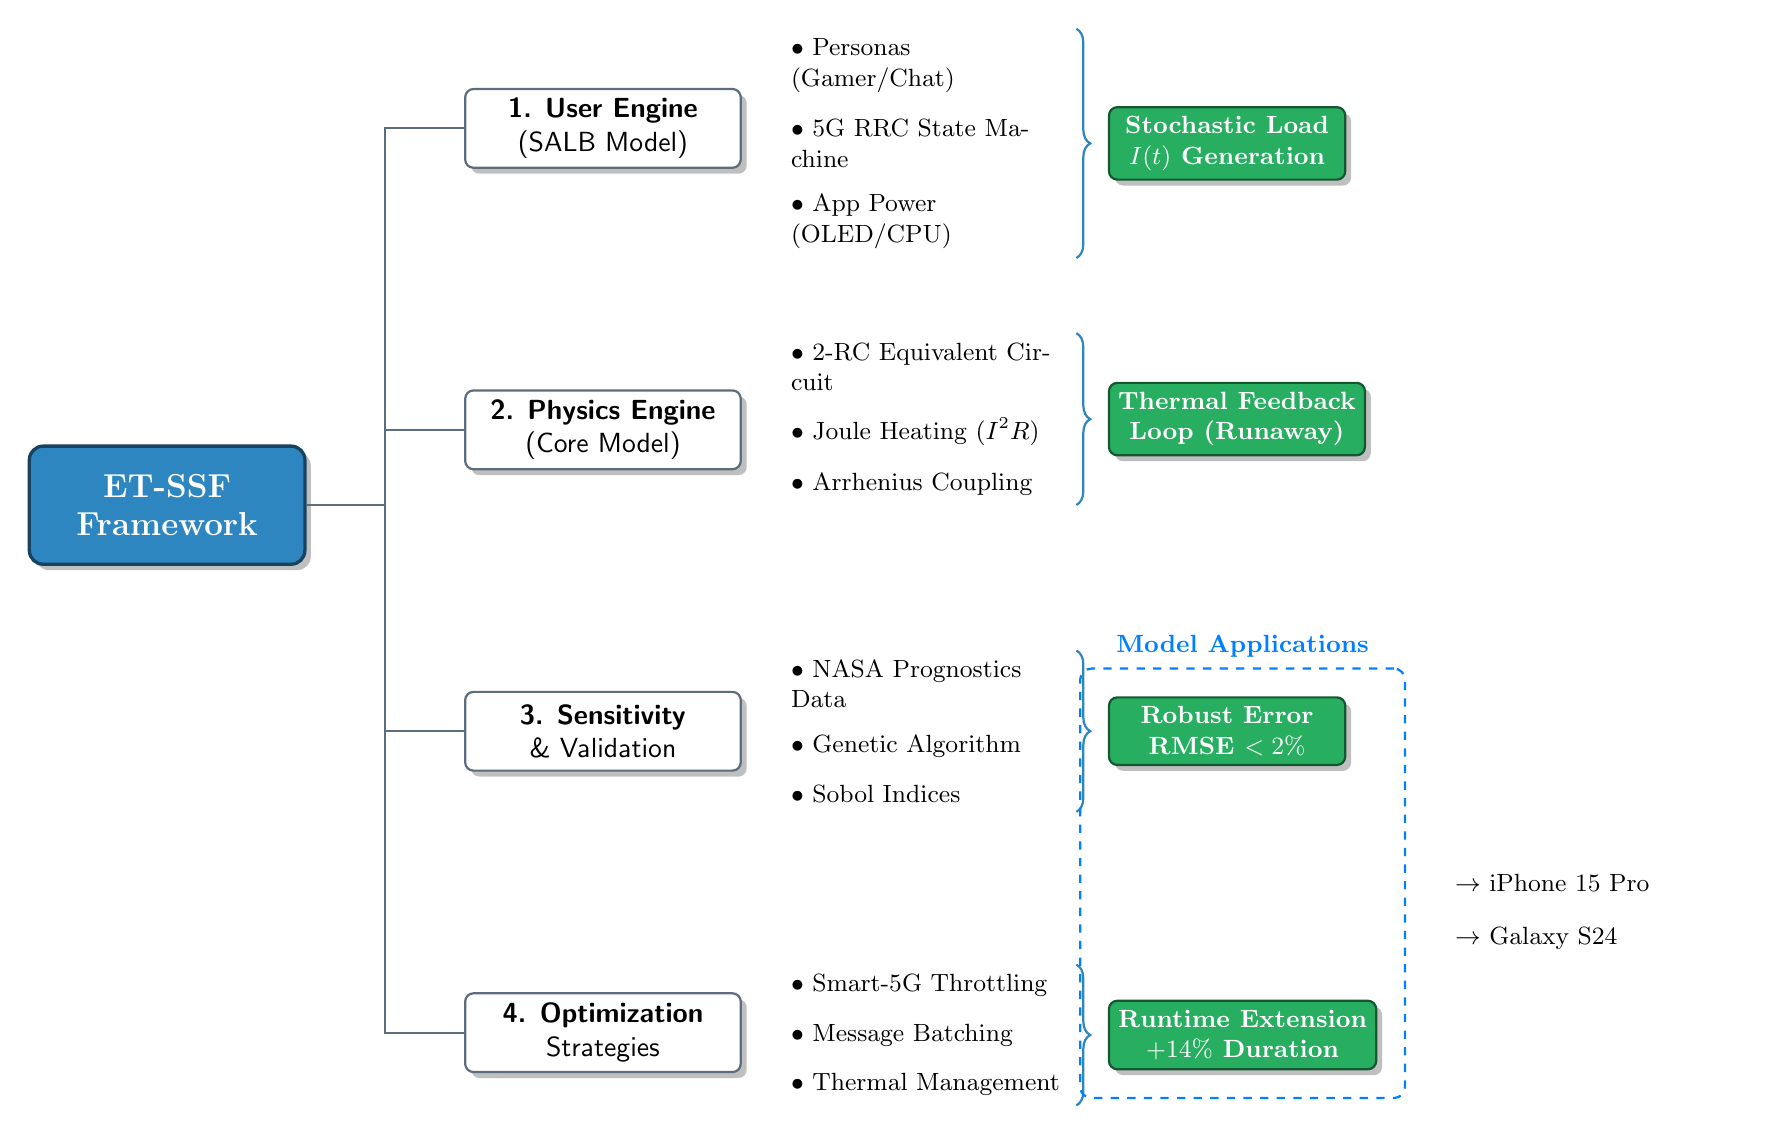
\begin{tikzpicture}[
    node distance=1.5cm and 1.5cm,
    font=\sffamily,
    % Root Node Style
    root/.style={
        rectangle, 
        rounded corners=5pt, 
        fill=rootBlue, 
        draw=rootBlue!50!black, 
        text=white, 
        very thick, 
        minimum width=3.5cm, 
        minimum height=1.5cm, 
        align=center, 
        drop shadow,
        font=\large\bfseries
    },
    % Level 1 Branch Nodes (Category Headers)
    branch/.style={
        rectangle, 
        rounded corners=3pt, 
        fill=white, 
        draw=borderGray, 
        thick, 
        minimum width=3.5cm, 
        minimum height=1.0cm, 
        align=center, 
        drop shadow
    },
    % Level 2 Item Nodes (Text lists)
    item/.style={
        text width=3.5cm, 
        align=left, 
        font=\small,
        anchor=west
    },
    % Outcome Nodes (Green Boxes)
    outcome/.style={
        rectangle, 
        rounded corners=3pt, 
        fill=accentGreen, 
        draw=accentGreen!50!black, 
        text=white, 
        thick, 
        align=center, 
        minimum width=3cm, 
        drop shadow,
        font=\small\bfseries
    },
    % Connecting Lines
    line/.style={
        draw=borderGray, 
        thick
    },
    % Brace Style
    brace/.style={
        draw=rootBlue, 
        thick, 
        decoration={brace, amplitude=5pt, mirror}, 
        decorate
    }
]

% --- ROOT NODE ---
\node[root] (Center) {ET-SSF\\Framework};

% --- BRANCH 1: USER ENGINE (Top) ---
\node[branch, above right=3.5cm and 2cm of Center] (UserEngine) {\textbf{1. User Engine}\\(SALB Model)};
% Items
\node[item, right=0.5cm of UserEngine, yshift=0.8cm] (UserItems1) {$\bullet$ Personas (Gamer/Chat)};
\node[item, below=0.1cm of UserItems1] (UserItems2) {$\bullet$ 5G RRC State Machine};
\node[item, below=0.1cm of UserItems2] (UserItems3) {$\bullet$ App Power (OLED/CPU)};
% Brace and Outcome
\draw[brace] (UserItems3.south east) -- (UserItems1.north east) coordinate[midway, xshift=0.2cm] (Brace1);
\node[outcome, right=0.2cm of Brace1] (CurrentOut) {Stochastic Load\\$I(t)$ Generation};

% --- BRANCH 2: PHYSICS ENGINE (Middle Top) ---
\node[branch, below=2.8cm of UserEngine] (PhysicsEngine) {\textbf{2. Physics Engine}\\(Core Model)};
% Items
\node[item, right=0.5cm of PhysicsEngine, yshift=0.8cm] (PhysItems1) {$\bullet$ 2-RC Equivalent Circuit};
\node[item, below=0.1cm of PhysItems1] (PhysItems2) {$\bullet$ Joule Heating ($I^2R$)};
\node[item, below=0.1cm of PhysItems2] (PhysItems3) {$\bullet$ Arrhenius Coupling};
% Brace and Outcome
\draw[brace] (PhysItems3.south east) -- (PhysItems1.north east) coordinate[midway, xshift=0.2cm] (Brace2);
\node[outcome, right=0.2cm of Brace2] (FeedbackOut) {Thermal Feedback\\Loop (Runaway)};

% --- BRANCH 3: VALIDATION (Middle Bottom) ---
\node[branch, below=2.8cm of PhysicsEngine] (Validation) {\textbf{3. Sensitivity}\\ \& Validation};
% Items
\node[item, right=0.5cm of Validation, yshift=0.6cm] (ValItems1) {$\bullet$ NASA Prognostics Data};
\node[item, below=0.1cm of ValItems1] (ValItems2) {$\bullet$ Genetic Algorithm};
\node[item, below=0.1cm of ValItems2] (ValItems3) {$\bullet$ Sobol Indices};
% Brace and Outcome
\draw[brace] (ValItems3.south east) -- (ValItems1.north east) coordinate[midway, xshift=0.2cm] (Brace3);
\node[outcome, right=0.2cm of Brace3] (ValOut) {Robust Error\\RMSE $< 2\%$};

% --- BRANCH 4: STRATEGIES (Bottom) ---
\node[branch, below=2.8cm of Validation] (Strategies) {\textbf{4. Optimization}\\Strategies};
% Items
\node[item, right=0.5cm of Strategies, yshift=0.6cm] (StratItems1) {$\bullet$ Smart-5G Throttling};
\node[item, below=0.1cm of StratItems1] (StratItems2) {$\bullet$ Message Batching};
\node[item, below=0.1cm of StratItems2] (StratItems3) {$\bullet$ Thermal Management};
% Brace and Outcome
\draw[brace] (StratItems3.south east) -- (StratItems1.north east) coordinate[midway, xshift=0.2cm] (Brace4);
\node[outcome, right=0.2cm of Brace4] (StratOut) {Runtime Extension\\$+14\%$ Duration};

% --- CONNECTIONS ---
% Draw lines from Root to Branches
\draw[line] (Center.east) -- ++(1cm,0) |- (UserEngine.west);
\draw[line] (Center.east) -- ++(1cm,0) |- (PhysicsEngine.west);
\draw[line] (Center.east) -- ++(1cm,0) |- (Validation.west);
\draw[line] (Center.east) -- ++(1cm,0) |- (Strategies.west);

% --- EXTENSIONS (Dashed Box for Case Studies like the image) ---
% Let's add the "Device Comparison" box on the far right
\node[draw=blue!50!cyan, dashed, thick, rounded corners, fit=(ValOut) (StratOut), inner sep=10pt, label={[blue!50!cyan, font=\small\bfseries]above:Model Applications}] (Box) {};
\node[item, right=0.5cm of Box.east, anchor=west] (App1) {$\to$ iPhone 15 Pro};
\node[item, below=0.2cm of App1] (App2) {$\to$ Galaxy S24};

\end{tikzpicture}
\end{document}
